\documentclass[class=jsarticle, crop=false, dvipdfmx, fleqn]{standalone}
%% preamble for Numerical-structure-analysis report

\input{/Users/User/Documents/Project/TeX/preamble/mypreamble}

%% titles
\title{先端データ解析論 レポート}
\author{37-196360 \quad 森田涼介}


%% setting for listings
\newtcbinputlisting[auto counter]{\reportlisting}[3][]{%
	listing file = {#3},
	listing options = {language=python, style=tcblatex, numbers=left, numberstyle=\tiny},
	listing only,
	breakable,
	toprule at break = 0mm,
	bottomrule at break = 0mm,
	left = 6mm,
	sharp corners,
	drop shadow,
	title = Listings \thetcbcounter : \texttt{#2},
	label = #1,
	}



%% title format
\usepackage{titlesec}
\titleformat{\section}{\LARGE}{宿題\thesection}{0zw}{}
\newcommand{\sectionbreak}{\clearpage}
\titleformat{\subsection}{\Large}{\Alph{subsection})}{0zw}{}

\begin{document}
\section{}

ガウスカーネルモデル
\begin{align}
    & f_{\bm{\theta}} (\bm{x})
        = \sum_{j=1}^{n+n'} \theta_j K(\bm{x},\ \bm{x}_j)
        = \bm{K} \bm{\theta} \\
    & K(\bm{x},\ \bm{c}) = \exp(- \frac{||\bm{x} - \bm{c}||^2}{2 h^2}) \\
    & \bm{K} =
        \begin{bmatrix}
            K(\bm{x}_1,\ \bm{x}_1) & \cdots & K(\bm{x}_{n+n'},\ \bm{x}_1) \\
            \vdots & \ddots & \vdots \\
            K(\bm{x}_{n+n'},\ \bm{x}_1) & \cdots & K(\bm{x}_{n+n'},\ \bm{x}_{n+n'})
        \end{bmatrix}
\end{align}
に対してラプラス正則化最小二乗分類を実装する。
\begin{align}
    & \sum_{i,\ i' = 1}^{m} W_{i,\ i'} (a_i - a_{i'})^2 = 2 \sum_{i,\ i' = 1}^{m} L_{i,\ i'} a_i a_{i'} \\
    & \bm{D} = \mathrm{diag}\qty(\sum_{i=1}^{m} W_{1,\ i},\ \cdots,\ \sum_{i=1}^{m} W_{m,\ i}) \\
    & \bm{L} = \bm{D} - \bm{W}
\end{align}
近傍グラフの重みにはガウスカーネルを用い,
\begin{equation}
    W_{i,\ i'} = \exp(- \frac{||\bm{x}_i - \bm{x}_{i'}||^2}{2 h^2})
\end{equation}
とする。

目的関数は,
\begin{align}
    J(\bm{\theta})
        & = \sum_{i=1}^{n} \qty(f_{\bm{\theta} (\bm{x}_i) - y_i})^2
            + \lambda ||\bm{\theta}||^2
                + \nu \sum_{i,\ i' = 1}^{n+n'} W_{i,\ i'} (f_{\bm{\theta}} (\bm{x}_i) - f_{\bm{\theta}} (\bm{x}_{i'}))^2 \\
        & = ||\tilde{\bm{K}} \bm{\theta} - \bm{y}||^2
            + \lambda ||\bm{\theta}||^2
            + 2 \nu \bm{\theta}^\mathrm{T} \bm{K}^\mathrm{T} \bm{L} \bm{K} \bm{\theta}
\end{align}
となる。
これを\(\bm{\theta}\)で偏微分すると,
\begin{align}
    \pdv{J}{\bm{\theta}}
        & = 2 \tilde{\bm{K}}^\mathrm{T} \tilde{\bm{K}} \bm{\theta}
            - 2 \tilde{\bm{K}} \bm{y}
            + 2 \lambda \bm{\theta}
            + 4 \nu \bm{K}^\mathrm{T} \bm{L} \bm{K} \bm{\theta} \\
        & = 2 \qty(\tilde{\bm{K}}^\mathrm{T} \tilde{\bm{K}} + \lambda \bm{I} + 2 \nu \bm{K}^\mathrm{T} \bm{L} \bm{K}) \bm{\theta}
            - 2 \tilde{\bm{K}} \bm{y} \\
        & = \bm{0}
\end{align}
これより,
\begin{equation}
    \hat{\bm{\theta}}
        = \arg\min_{\bm{\theta}} J(\bm{\theta})
        = \qty(\tilde{\bm{K}}^\mathrm{T} \tilde{\bm{K}} + \lambda \bm{I} + 2 \nu \bm{K}^\mathrm{T} \bm{L} \bm{K})^{-1} \tilde{\bm{K}} \bm{y}
\end{equation}
である。

\(h = 1.0,\ \lambda = 1.0,\ \nu = 1.0\)として
これを実装したものが\pageref{listing:assignment1}ページのListing \ref{listing:assignment1}である。

結果は図\ref{fig:result}に示した通りである。
教師ありのデータは各クラス1つずつしかないが,
ラベルなしのデータについても上手く分けられている。


\begin{figure}[H]
    \centering
    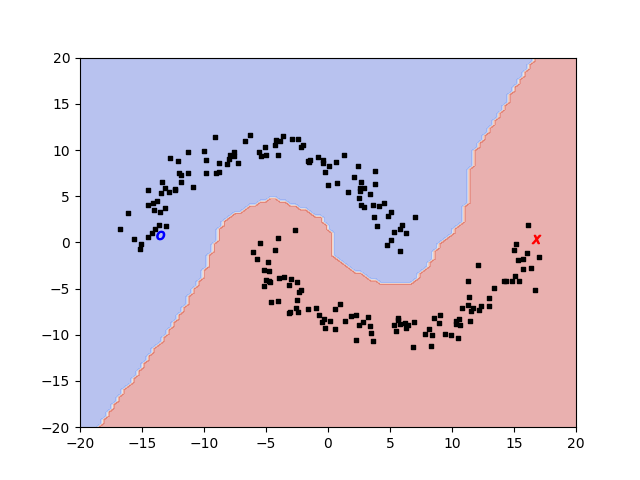
\includegraphics[clip, width=12cm]{../figures/assignment1_result}
    \caption{結果}
    \label{fig:result}
\end{figure}


\end{document}
